\documentclass[../main.tex]{subfiles}
\begin{document}
\section{Introduction}

Residential segregation, the uneven distribution of ethnic groups within a confined geographic area, has long been of interest to both scholars and policymakers. Segregation is a salient feature of Danish society, yet there remains limited evidence of how ethnic background matters for residential sorting. Does it matter and if so, by how much?

%Despite this, limited evidence exists of how ethnic neighborhood composition directly affects the decision to move. This likely reflects the complexity involving credible identification of the importance of neighbor identity.

\textcite{schelling1971dynamic} remains the foundational piece in the literature on theoretical determinants of segregation. The key prediction of \textcite{schelling1971dynamic} is that neighborhoods may experience a rapid outflow of residents belonging to a majority, or "tip", when the share of (new) residents belonging to a minority reach a certain threshold. \textcite{schelling1971dynamic} noted that this phenomenon may happen even if majority residents are relatively tolerant of other minorities. Like \textcite{schelling1971dynamic}, I focus on the \textit{third} kind of segregation - individually motivated segregation as opposed to either the more organized or economically induced kind. For instance, clustering by similar income or education is an example of the latter, while the Jim Crow laws, though rather extreme, is an example of the former. I do not make the claim that organized or economically induced segregation do not exist or play a role in Denmark (perhaps less so than in the United States), but that individual preferences, even if it is not the main driver of observed segregation, still matters and deserves attention. 

Perhaps most similar to me is \textcite{rockwool_boje2024immigrants}, who examine native flight in Denmark, both at the neighborhood and building level. They find that an increase in 30 percentage points in the share of non-Western foreigners increase the propensity for natives to move out in any given year by around 8 pct.\footnote{The definition of neighborhoods by \textcite{rockwool_boje2024immigrants} follows \textcite{damm2008danish} and totals 2,296.} 

Identifying the importance of individual preferences for neighborhood composition is vital to understand. It has been widely established that neighborhoods, both who live there and amenities within, matter for long-run outcomes. For instance, \textcite{chetty2016effects} show the positive impact on earnings and college attendance when presented with the opportunity to move to a more affluent neighborhood. In a Danish context, \textcite{hasager2024sick_poor_neighborhood} show the importance of neighborhood (both at the building and parish level) composition on long-term health outcomes using the quasi-experiment of the Danish Spatial Policy for refugee placement. \textcite{damm2014crime} use the same policy as part of their empirical framework and finds that neighborhood crime rates is strongly associated with youth criminal behavior.  

Work by \textcite{schelling1971dynamic} has spawned a rich literature on segregation from which many papers draw their inspiration from.  \textcite{card2008tipping} employ a single "tipping point" Schelling model in an RDD setting. They find discontinuity in the rate of change in minority shares ranging between 5 pct. (Portland, Oregon) to around 20 pct. (Los Angeles, California). \textcite{blair2017outside} further explores this concept, arguing that while points have increased over time, the outside option available to white households matter more to the patterns of segregation than the identity of their neighbors.

Inspired by \textcite{card2008tipping},\textcite{bohlmark_willen_2020_tipping} estimate tipping points in Sweden's largest cities (Stockholm, Malmo and Gothenburg) that range between 17-19 pct. Additionally, some evidence of spatial sorting \textcite{}


"Tipping behavior" has been frequently analyzed in the US (\textcite{Ananat_2011, davis2018long, chetty2015impacts}), but less so in Europe (\textcite{bohlmark_willen_2020_tipping}), let alone Denmark. 

In this paper, I aim to credibly estimate how households respond directly to receiving a new different-type neighbor.


The paper is structured as follows. 

\subsection{Definitions}
\label{sec:intro_definitions}
In the paper, I define 3 mutually exclusive types of households. (i) \textit{Native} households, where all members are of Danish origin; (ii) \textit{Non-West} households, where at least one member is of non-West origin and (iii) \textit{Western} households, where at least one household member is non-Native and of Western origin, but with no members that have \textit{non-Western} origin. I follow the definition of West/non-West countries by \textcite{west_non_west_def_dst}.
\end{document}







% 1) Determine treat/control
% - Treat: New non-West among K=3
% - Control: New non-west among K=4,..,40? 
% - Drop everyone else
% 2) Make panel. use lf.join_where(pl.date_range(..., eager=True)
% 3) Take unique ID's and collect
% - Inc, edu, emp
% 4) just have a little looksy @ BBR / DAR

%Section \ref{sec:model} outlines and  simulates a simplified of the Schelling model. Section \ref{sec:data} describes the data used in this paper. The empirical strategy is presented in Section \ref{sec:empirical_strategy}. The main results, including a heterogeneity analysis (?), are presented in Section \ref{sec:results}. In Section \ref{sec:Discussion}, I discuss some stuff(?). In Section \ref{sec:conclusion} I summarize and conclude.
Cont...

Include some stats:

\begin{figure}[H]
\centering
\caption{Different-type neighbors}
    \begin{subfigure}{0.47\textwidth}	
	\centering
    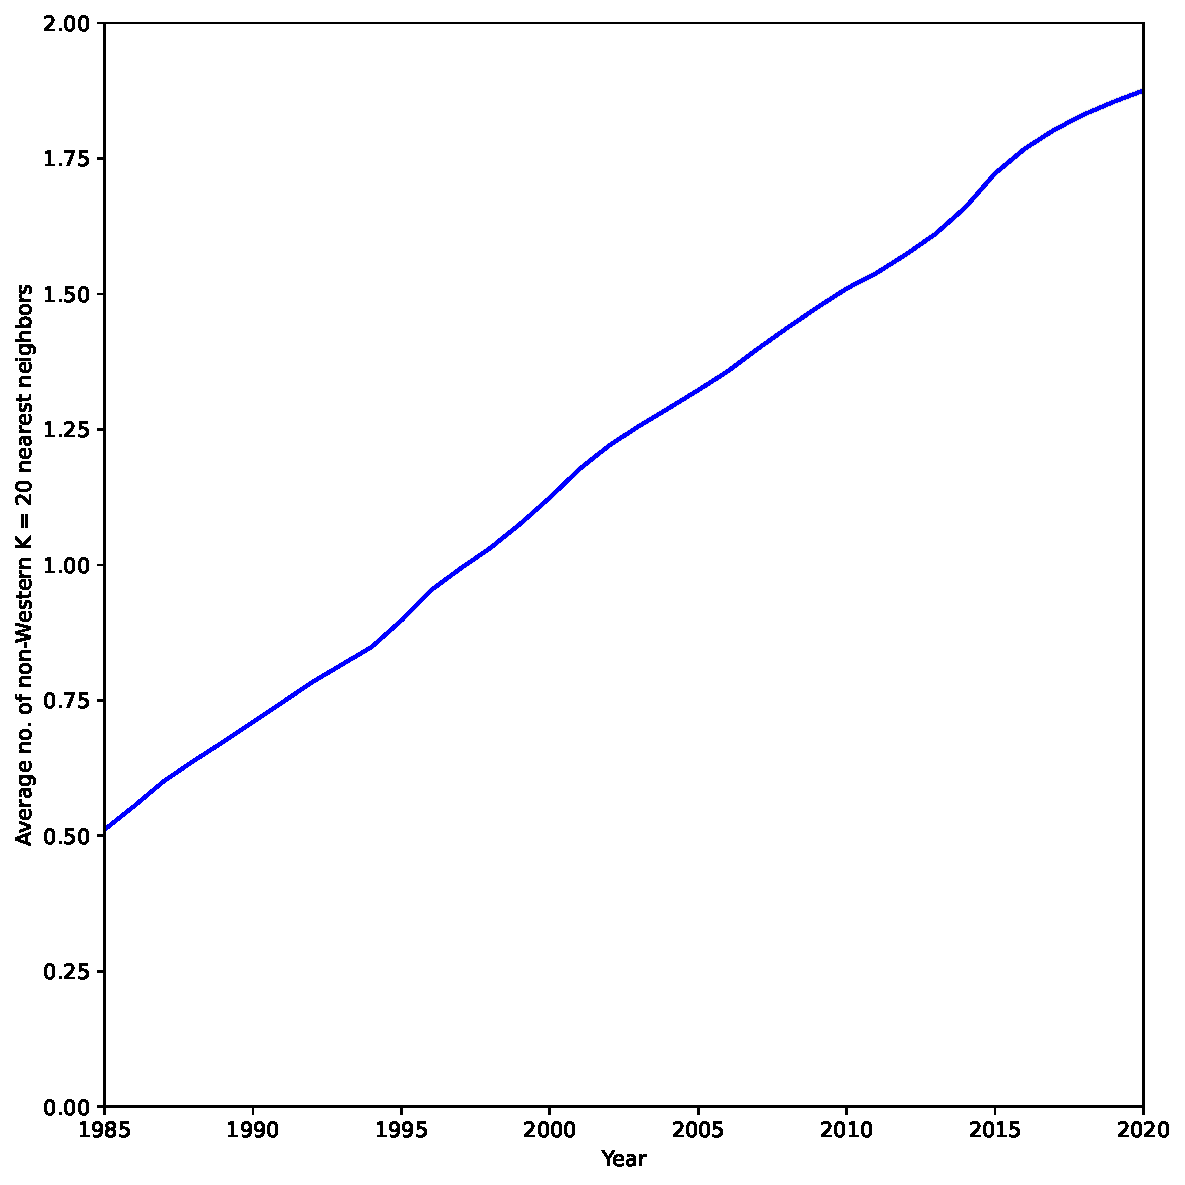
\includegraphics[width=\linewidth]{figs/mix_non_west_pos_nn_1985_2020.pdf}
	\caption{Non-Western neighbors} 
	\end{subfigure}	
    \begin{subfigure}{0.47\textwidth}	
	\centering
    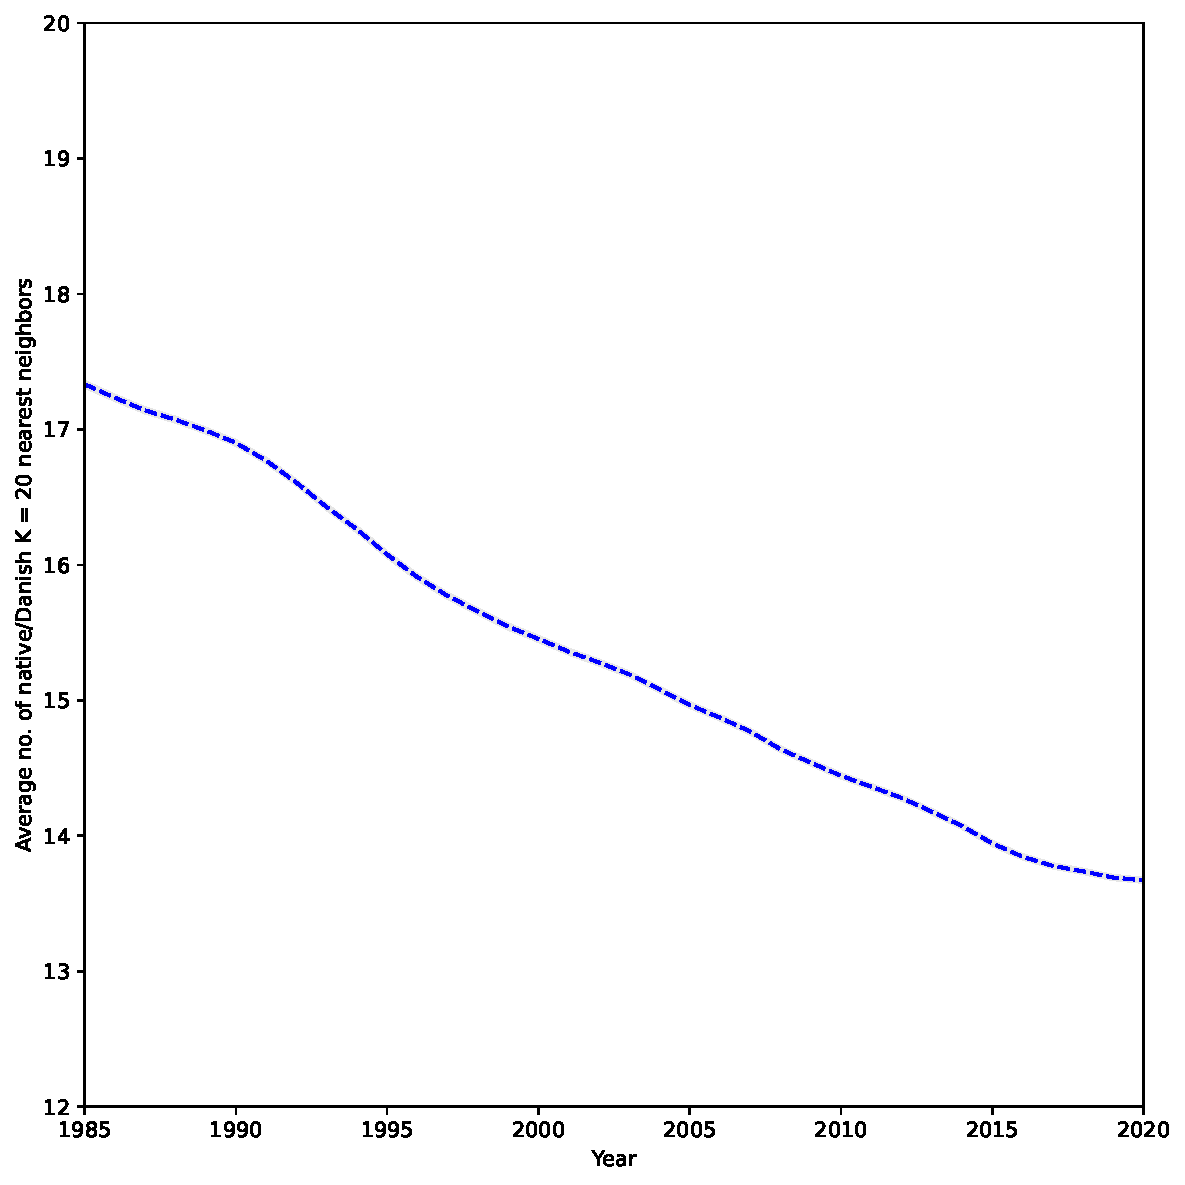
\includegraphics[width=\linewidth]{figs/native_nn_1985_2020.pdf}
	\caption{Danish/native neighbors} 
	\end{subfigure}	
      
    \label{fig:avg_k_nearest_dk}
    \begin{minipage}{.9\linewidth}
        \footnotesize \textit{Note}: Non-Western households refers to households where at least one household member is of non-Western origin. Danish/native households refers to households where all members is of Danish descent.
    \end{minipage}
\end{figure}

Some figures yet to be determined where to place can be found in Appendix \ref{sec:appendix_figs}
